\chapter{Straight Line}


\section{Gradient Revision and Equation of a Straight Line}
The gradient is the line's steepness. The bigger the number, the steeper it is. Its symbol is $m$.

Its equation is
\begin{equation*}
m = \frac{\text{vertical distance}}{\text{horizontal distance}}
\end{equation*}
or
\begin{equation}
m = \frac{y_2-y_1}{x_2-x_1}
\end{equation}

If the line is vertical ($\vert$), then it has an undefined gradient, e.g. when $x=1$. If it is horizontal (—), then $m=0$, e.g. when $y=1$.

From National 5, it should be known that, given a point and gradient, the equation of a line can be written using

\begin{equation}
y-b=m(x-a).
\end{equation}

\subsection{Example}
If $m=3$ and the line goes through point (-2,3), find the equation of the line.

\begin{align*}
y-b&=m(x-a)\\
y-3&=3(x+2)\\
y&=3(x+2)+3\\
y&=3x+6+9\\
y&=3x+9\\
\end{align*}

Note that the equation can be left in any form, no extra marks are awarded for leaving it in the form $0 = 3x - y + 9$


\section{$m=\tan\theta$}

\begin{figure}[h!]
	\centering
	\begin{tikzpicture}% function
		\begin{axis}
		[
			xlabel=$x$,
			ylabel=$y$,
			axis lines = left, % Only show axis on the left and bottom.
			axis equal,
			ymin = 0,
			xmin = 0,
		]
		\pgfplotsset{ticks=none}
		\addplot
		[
			samples = 100,
			color = black,
		]{sqrt(3)*x};
		\end{axis}
	\end{tikzpicture}
	\caption{Here, $\theta$ is 60$^\circ$.}
	\label{fig:mtan60}
\end{figure}
$\theta$ is the (in figure \ref{fig:mtan60} an acute) angle made from the $x$-axis in an anti-clockwise direction (also called in the positive direction of the $x$-axis). If $\theta$ is known, the gradient of the line can be found, and vice versa, by using

\begin{equation}
	m=\tan\theta
\end{equation}

\subsection{Examples}
\begin{enumerate}
	\item
	A line makes an angle of 120$^\circ$ with the positive direction of the $x$-axis. Find its gradient.
	
	One could just enter 120$^\circ$ into their calculator and get the right answer, but the following is a method of working it out if the question would appear in a non-calculator paper.
	\begin{align*}
	m&=\tan\theta\\
	&=\tan120^\circ\\
	&=-\tan60\\
	&=-\sqrt{3}
	\end{align*}
	
	\item
	A line's gradient is $-2$. Find the angle it makes in the positive direction of the $x$-axis.
	\begin{align*}
	\text{If $m=2$,}\\
	\tan\theta&=2\\
	\theta&=\tan^{-1}2\\
	&=63.43...\\
	\text{Now the proper line where $m=-2$,}\\
	\theta&=180-63.43...\\
	&=116.56...\\
	&\approx116.6^\circ
	\end{align*}

\end{enumerate}


\section{Perpendicular Lines ($\perp$)}
Perpendicular lines sit at right angles to each other. If lines are perpendicular, then
\begin{equation}
m_1 m_2 = -1.
\end{equation}

\subsection{Examples}
If two lines are perpendicular, calculate $m_1$ if $m_2$ is
\begin{enumerate}
	\item 6
	\item -7
	\item $\frac{2}{7}$
\end{enumerate}

\begin{enumerate}
	\item
	\begin{align*}
	m_1 m_2 &= -1\\
	3m_1 &= -1\\
	m_1&=-\frac{1}{3}
	\end{align*}
	
	\item
	\begin{align*}
	m_1 m_2 &= -1\\
	-7m_1 &= -1\\
	m_1&=\frac{1}{7}
	\end{align*}
	
	\item
	\begin{align*}
	m_1 m_2 &= -1\\
	\frac{2}{7}m_1 &= -1\\
	2m_1&=-7\\
	m_1&=-\frac{7}{2}
	\end{align*}
\end{enumerate}

As a shortcut, take the recipricol and change the sign.

\begin{enumerate}
	\setcounter{enumi}{3}
	\item
	Find the equation of the line perpendicular to $y=-\frac{2}{3}x+5$ that passes through the point $\left(1,7\right)$.

	\begin{align*}
		m &= -\frac{2}{3} & m_\perp &= \frac{3}{2}
	\end{align*}

	Now that the gradient of the perpendicular line has been found, it can be used in the equation.
	
	\begin{align*}
		y-b&=m(x-a)\\
		y-7&=\frac{3}{2}(x-1)\\
		y&=\frac{3}{2}x - \frac{3}{2} + 7\\
		y&=\frac{3}{2}x + \frac{11}{2}
	\end{align*}
\end{enumerate}


\section{Mid Point Formula}
To find the point in the middle of a line, use
\begin{equation}
\text{mid point} = \left(\frac{x_1 + x_2}{2},\frac{y_1 + y_2}{2}\right)
\end{equation}

\subsection{Examples}
\begin{enumerate}
	\item
	Find the mid point of $\left(1,-4\right)$ and $\left(7,8\right)$.
	
	\begin{align*}
		\text{mid point} &= \left(\frac{x_1 + x_2}{2},\frac{y_1 + y_2}{2}\right)\\
		&= \left(\frac{1 + 7}{2},\frac{-4 + 8}{2}\right)\\
		&= \left(4,2\right)
	\end{align*}
	
	\item
	\begin{figure}[h!]
		\centering
		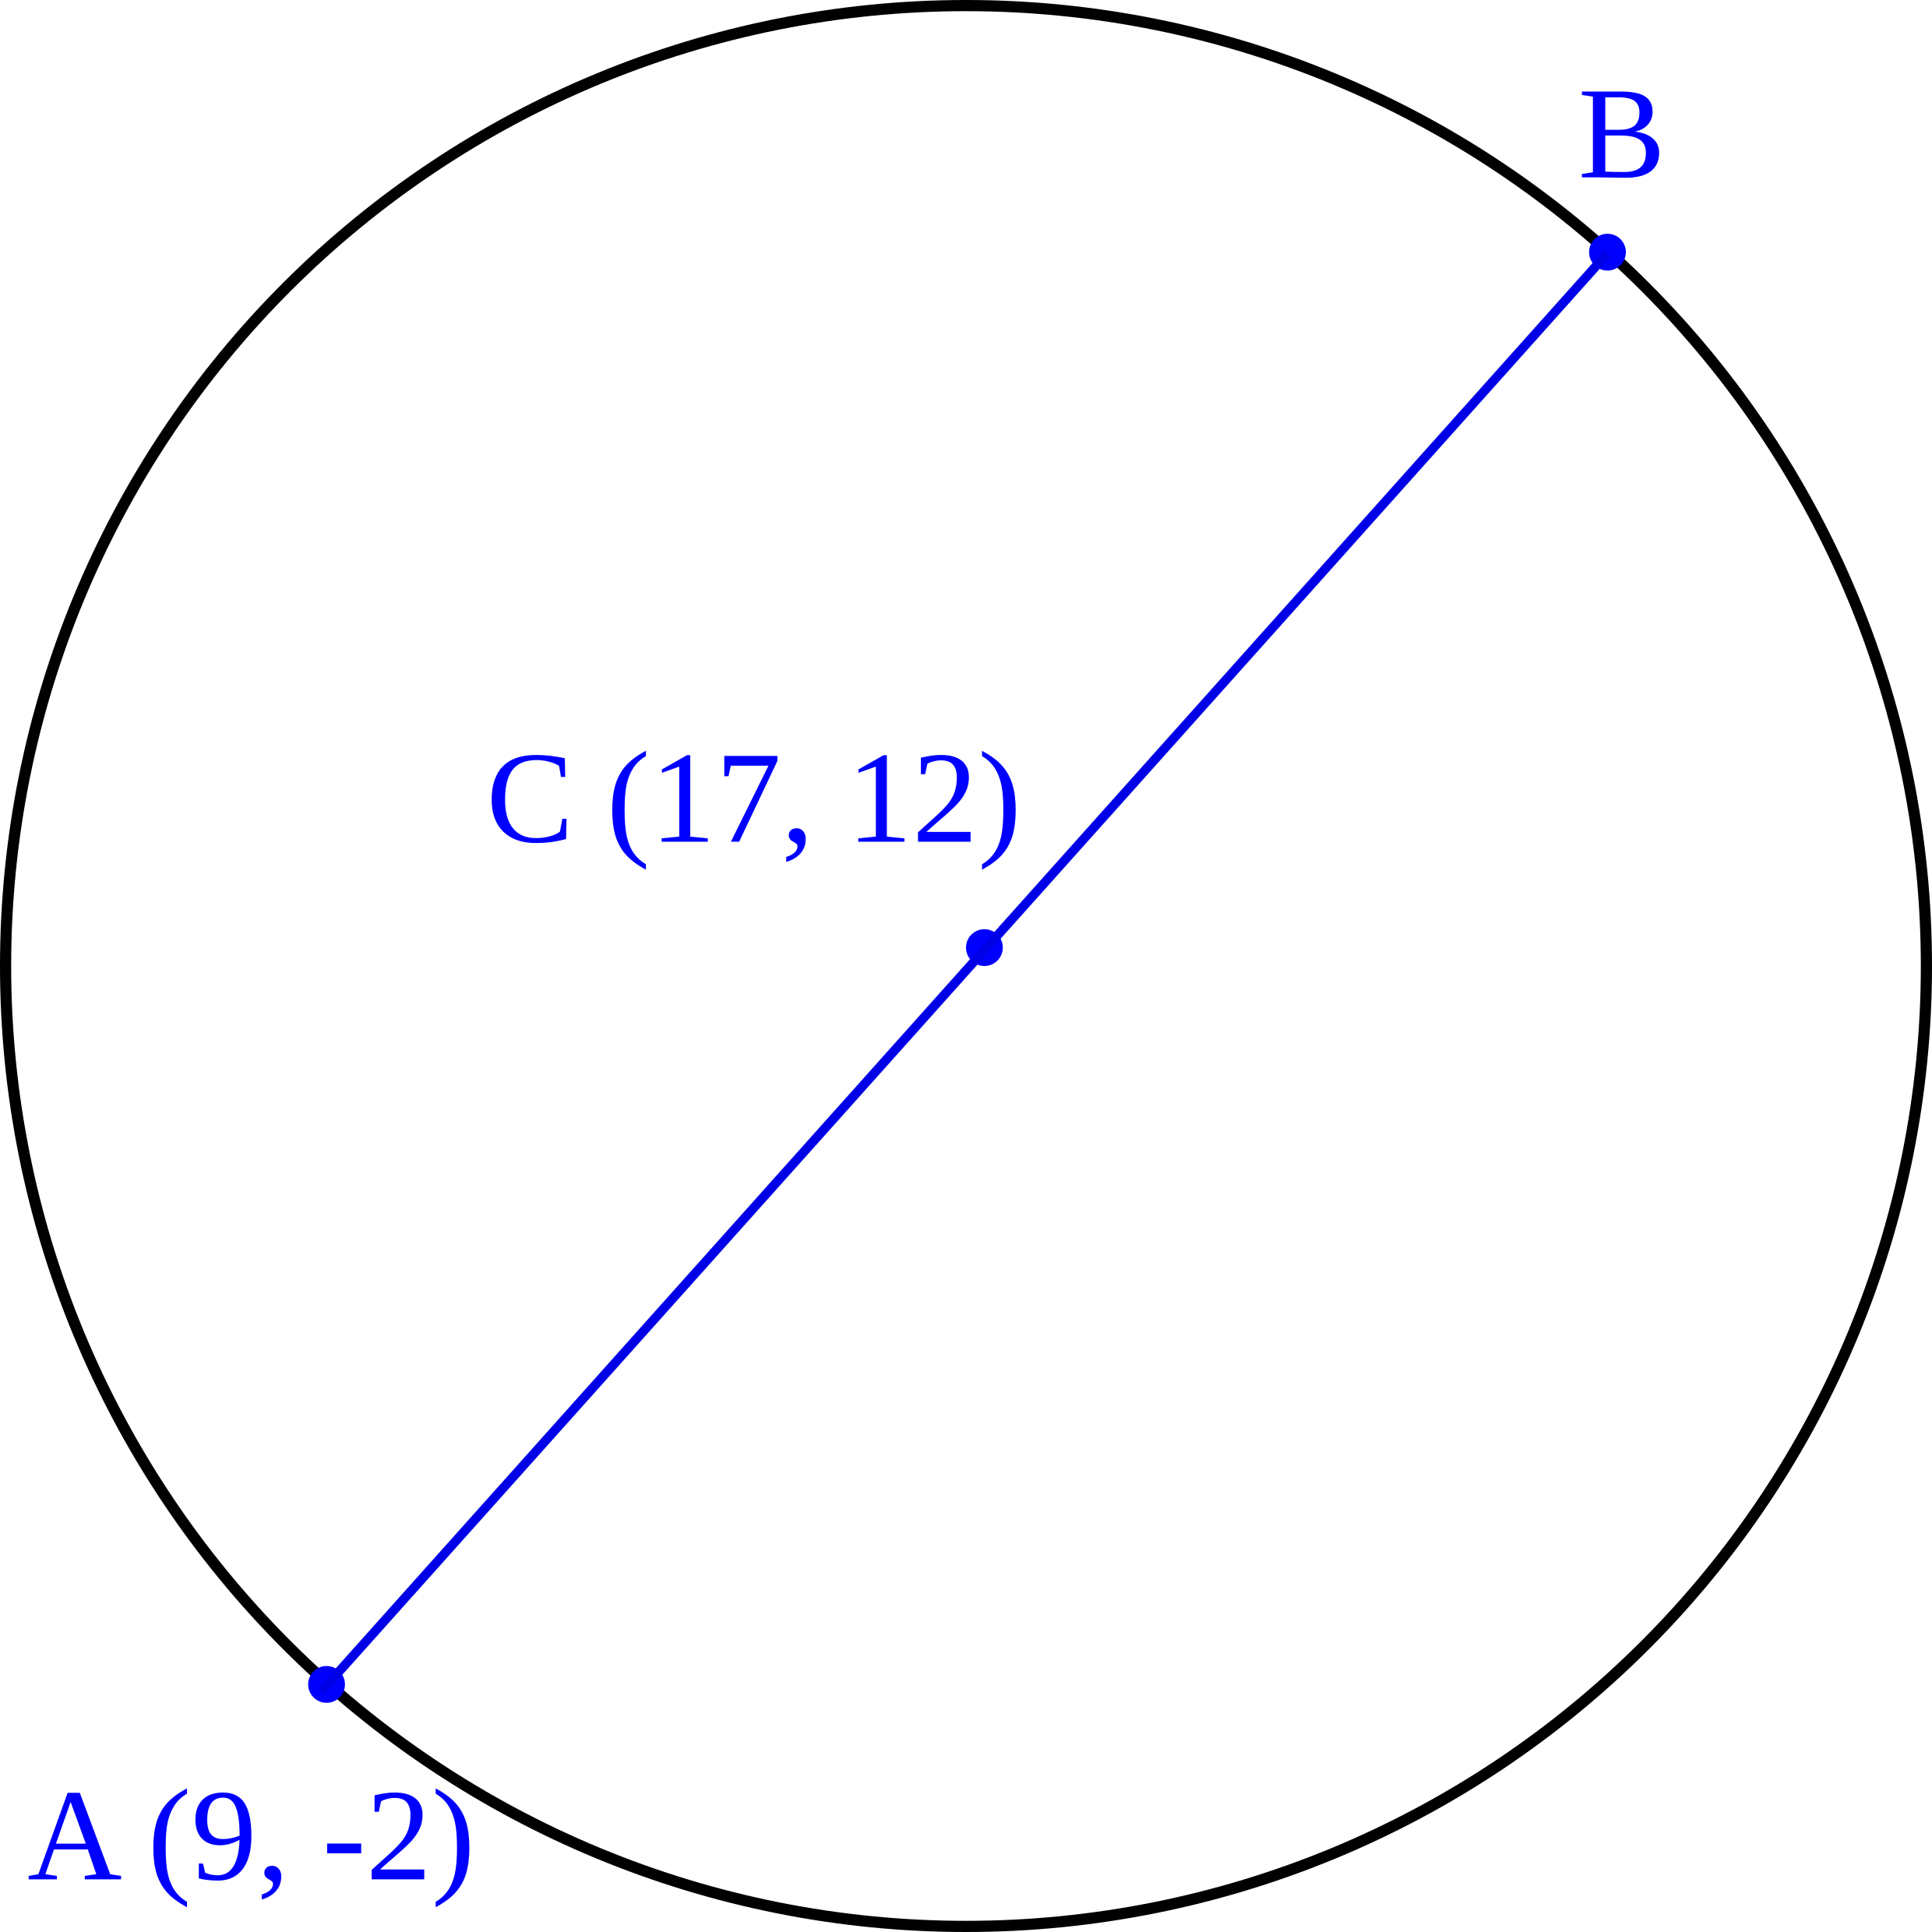
\includegraphics[width=0.5\linewidth]{images/MidPointQ2.png}
		\caption{Not to scale.}
		\label{fig:MidPointQ2}
	\end{figure}
	A circle has centre point $\left(17, 12\right)$. Two points $A(9, -2)$ and $B$ are drawn on its circumference, these are connecting by a diameter (see figure \ref{fig:MidPointQ2}). Find the coordinates of B.
	\begin{align*}
		\text{mid point} &= \left(\frac{x_1 + x_2}{2},\frac{y_1 + y_2}{2}\right)\\
		\left(17, 12\right) &= \left(\frac{9+x}{2},\frac{-2 + y_2}{2}\right)
	\end{align*}
	\begin{align*}
		\frac{9+x}{2} &= 17 & \frac{-2+y}{2} &= 12\\
		9+x &= 34 & -2+y &= 24\\
		x &= 25 & y &= 26
	\end{align*}
	
	So the coordinate of B is $\left(25,26\right)$.
\end{enumerate}


\section{Collinearity}
Points that are collinear lie on a straight line.

\begin{figure}[h!]
	\centering
	\begin{subfigure}[b]{0.4\linewidth}
		\begin{tikzpicture}% coordinates
		\begin{axis}
		[
			axis equal,
			axis line style={draw=none},
		]
		\pgfplotsset{ticks=none} % Get rid of numbers and ticks.
		\addplot
		[
			color=black,
			mark=*,
		] coordinates
		{
			(3,0)(6,1)(9,2)
		};
		\end{axis}
		\end{tikzpicture}
		\caption{Collinear.}
	\end{subfigure}
	\begin{subfigure}[b]{0.4\linewidth}
		\begin{tikzpicture}% coordinates
		\begin{axis}
		[
			axis equal,
			axis line style={draw=none},
		]
		\pgfplotsset{ticks=none} % Get rid of numbers and ticks.
		\addplot
		[
			color=black,
			mark=*,
		] coordinates
		{
			(1,0)(2,1)(7,2)
		};
		\end{axis}
		\end{tikzpicture}
		\caption{Not collinear.}
	\end{subfigure}
	\caption{Examples of collinearity.}
	\label{fig:collinearityExample}
\end{figure}

To test for collinearity of three points $A,B,C$:
\begin{enumerate}
	\item find $m_{AB}$,
	\item find $m_{BC}$,
	\item if $m_{AB}=m_{BC}$, then (because $B$ is a common point) they are collinear.
\end{enumerate}

\subsection{Examples}
\begin{enumerate}
	\item
	Show that the points $P\left(-6,-1\right), Q\left(0,2\right), R\left(8,6\right)$ are collinear.
	
	\begin{align*}
		m_{PQ}&=\frac{2+1}{0+6} & m_{QR}&=\frac{6-2}{8-0}\\
		&=\frac{3}{6} & &=\frac{4}{8}\\
		&=\frac{1}{2} & &=\frac{1}{2}
	\end{align*}
	Since $m_{PQ} = m_{QR}$, and $Q$ is a common point, $PQR$ are collinear.
	
	\item
	If $A\left(1,-1\right), B\left(-1,k\right), C\left(5,7\right)$ are collinear, find k.
	
	\begin{align*}
		m_{AB}&=m_{BC}\\
		\frac{k-(-1)}{-1-1}&=\frac{7-k}{5-(-1)}\\
		\frac{k+1}{-2}&=\frac{7-k}{6}\\
		6(k+1)&=-2(7-k)\\
		6k+6&=-14+2k\\
		4k&=-20\\
		k&=5
	\end{align*}
\end{enumerate}


\section{Median Lines}
\begin{figure}[h!]
	\centering
	\begin{tikzpicture}[scale=8]
		% Draw triangle.
		\coordinate[label=left:{$A$}] (a) at (0mm,0mm);		\coordinate[label=above:{$B$}] (b) at (7mm,5mm);		\coordinate[label=right:{$C$}] (c) at (10mm,1mm);
		\draw (a) -- (b) -- (c) -- cycle;
		
		% Draw point M.
		\coordinate
		[
			label=below:{$M$},
			circle,
			fill,
			color=blue,
			inner sep=1mm,
			scale=0.5
		] (m) at (5mm,0.5mm);
		
		% Connect point M and B.
		\draw[color=blue] (m) -- (b) -- cycle;
	\end{tikzpicture}
	\caption{Median from B.}
	\label{fig:median}
\end{figure}

The median is a line from a vertex of a triangle to the mid point of the opposite.

To find the median from $B$ in a triangle $ABC$ (such as in figure \ref{fig:median}):
\begin{enumerate}
	\item find the mid point of $AC$ (hereafter called $M$), since the opposite of $B$ is $AC$,
	\item find $m_{BM}$,
	\item use $y-b=m(x-a)$ with $B$ or $M$ and $m_{BM}$.
\end{enumerate}

\subsection{Example}
In $\triangle ABC$, $A(4,-9)$, $B(10,2)$, and $C(4,-4)$. Find the equation of the median from A.

\begin{align*}
	\text{mid point} &= \left(\frac{10+4}{2},\frac{2-4}{2}\right) & m_{AM} &= \frac{-1-(-9)}{7-4}\\
	&=\left(7,-1\right) & &= \frac{8}{3}
\end{align*}
\begin{align*}
	y-b&=m(x-a)\\
	y+9&=\frac{8}{3}\left(x-4\right)\\
	3y+27&=8\left(x-4\right)\\
	3y&=8x-32-27\\
	3y&=8x-59
\end{align*}


\section{Altitude}
\begin{figure}[h!]
	\centering
	\begin{tikzpicture}[scale=2]
		% Draw triangle.
		\coordinate[label=left:{$A$}] (a) at (0cm,0cm);		\coordinate[label=above:{$B$}] (b) at (1cm,2.5cm);		\coordinate[label=right:{$C$}] (c) at (2.5cm,0.5cm);
		\coordinate[] (q) at ($(c)!(b)!(a)$) {};
		\draw (a) -- (b) -- (c) -- cycle;
		\draw[color=blue] (b) -- (q);
		
		\tkzMarkRightAngle[radius=0.05cm](b,q,c)
	\end{tikzpicture}
	\caption{Altitude from B.}
	\label{fig:altitude}
\end{figure}

The altitude is a straight line form a vertex to the other side at right angles.

To find the altitude from $B$ in a triangle $ABC$ (such as in figure \ref{fig:altitude}):
\begin{enumerate}
	\item find $m_{AC}$,
	\item find $m_\perp$,
	\item use $y-b=m(x-a)$ with $m_\perp$ and $B$.
\end{enumerate}

\subsection{Example}
The triangle $ABC$ has vertices $A(3,-5)$, $B(4,3)$, and $C(-7,2)$. Find the altitude from A.

\begin{align*}
	m_{CB}&=\frac{3-2}{4-(-7)} & m_\perp&=-11\\
	&=\frac{1}{11}
\end{align*}
\begin{align*}
	y-b&=m(x-a)\\
	y+5&=-11(x-3)\\
	y&=-11x+33-5\\
	y&=-11x+28
\end{align*}


\section{Perpendicular Bisector}
\begin{figure}[h!]
	\centering
	\begin{tikzpicture}[scale=2]
		% Draw triangle.
		\coordinate[label=left:{$A$}] (a) at (0cm,0cm);		\coordinate[label=above:{$B$}] (b) at (4cm,0cm);		\coordinate[] (p) at (2cm,1cm);
		\coordinate[] (q) at (2cm,0cm);
		\coordinate[] (r) at (2cm,-1cm);
		\draw (a) -- (b);
		\draw[color=blue] (p) -- (r);
		
		\tkzMarkRightAngle[radius=0.05cm](p,q,b)
	\end{tikzpicture}
	\caption{The perpendicular bisector of $AB$ is here in blue.}
	\label{fig:pb}
\end{figure}

The perpendicular bisector (abbr. PB) is a line that cuts another line in the middle and sits at right angles.

To find the PB of a line $AB$:
\begin{enumerate}
	\item find the mid point $AB$,
	\item find $m_{AB}$,
	\item find $m_\perp$,
	\item use $y-b=m(x-a)$ with the mid point $AB$ and $m_\perp$.
\end{enumerate}

\subsection{Example}
Two points are $A(-2,1)$ and $B4,7)$ are connected by a line. Find the equation of the perpendicular bisector.

\begin{align*}
	\text{mid point} &= \left(\frac{-2+4}{2},\frac{1+7}{2}\right) & m_{AB} &= \frac{7-1}{4-(-2)} & m_\perp&=-1\\
	&=(1,4) & &=1
\end{align*}
\begin{align*}
	y-b&=m(x-a)\\
	y-4&=-1(x-1)\\
	y&=-x+1+4\\
	y&=-x+5
\end{align*}


\section{Intersection of Lines}
The point of intersection (abbr. POI) of two lines can be found through solving each line's equation simultaneously.

The National 5 course most likely focussed on the method of elimination, a better method is to use substitution. However, sometimes, such as in the second example, the equations are so simple that it would be stupid to not eliminate.

\subsection{Examples}
\begin{enumerate}
	\item
	Two lines have equations 2x-y+11=0 and x+2y-7 = 0. Find the point of intersection.
	
	\begin{align*}
		2x-y+11&=0\\
		y=&2x+11
	\end{align*}
	Sub $y=2x+11$ into $x+2y-7=0$,
	\begin{align*}
		x+2(2x+11)-7&=0\\
		x+4x+22-7&=0\\
		5x+15&=0\\
		5x&=-15\\
		x&=-3
	\end{align*}
	\begin{align*}
		y&=2x+11 & POI=(-3,5)\\
		y&=2(-3)+11\\
		&=-6+11\\
		&=5
	\end{align*}
	
	\item
	In triangle $ABC$ with points $A(1,0)$, $B(-4,3)$, $C(0,-1)$, find the median from A, the altitude from C, and henceforth the POI.
	
	\textit{Median from A:}
	\begin{align*}
		\text{mid point} &= \left(\frac{-4+0}{2},\frac{3+(-1)}{2}\right) & m &= \frac{3-0}{-4-1} \\
		&= (-2,1) & &=-\frac{1}{3}
	\end{align*}
	\begin{align*}
		y-b&=m(x-a)\\
		y-1&=-\frac{1}{3}\left(x+2\right)\\
		3y-3&=-\left(x+2\right)\\
		3y&=-x-2+3\\
		3y&=-x+1
	\end{align*}
	
	\textit{Altitude from C:}
	\begin{align*}
		m_{AB}&=\frac{3-0}{-4-1} & m_\perp&=\frac{5}{3} \\
		&=-\frac{3}{5}
	\end{align*}
	\begin{align*}
		y-b&=m(x-a)\\
		y+1&=\frac{5}{3}\left(x+0\right)\\
		3y+3&=5\left(x+0\right)\\
		3y&=5x-3
	\end{align*}
	
	\textit{Point of intersection:}
	\begin{align*}
		3y&=-x+1 & 3y&=-x+1\\
		\makebox[0pt][l]{\uline{\phantom{$--3y=5x-3$}}}
		-\;\;3y&=5x-3 & 3y&=-\frac{2}{3}+1\\
		0&=-6x+4 & 9y&=-2+3\\
		6x&=4 & 9y&=1\\
		x&=\frac{2}{3} & y=\frac{1}{9}\\
	\end{align*}
	\begin{equation*}
		POI = \left(\frac{2}{3},\frac{1}{9}\right)
	\end{equation*}
\end{enumerate}